\chapter{Algoritmo Evolutivo Híbrido Para o Escalonamento de Tarefas e Alocação de Arquivos}\label{chap5}

Este capítulo apresenta o AEH-ETAA, um algoritmo evolutivo híbrido que soluciona o problema de escalonamento de WfCs em ambientes de nuvens computacionais conforme o modelo matemático proposto neste trabalho. O algoritmo é apresentado  em função de seus principais métodos, discutidos em detalhes nas seções que seguem.



\section{AEH-ETAA}

Algoritmos Evolutivos (AE) \cite{Moraglio2012} são métodos de otimização inspirados nos mecanismos de evolução biológica observados na natureza. No AE, cada cromossomo é um indivíduo de uma população e representa uma possível solução para o problema. A busca pela melhor solução é guiada por uma função de \textit{fitness}, que atribui qualidade aos cromossomos. A cada iteração do algoritmo, novos indivíduos são gerados através da operação de \textit{crossover} e a diversidade da população é obtida através da função de mutação. Neste trabalho, um Algoritmo Evolutivo Hibrido (AEH) que combina os operadores do AE,  buscas locais e um método de \textit{path relinking} \cite{Reeves1998} foi desenvolvido. De acordo com Moscato e Cotta \cite{Moscato2010}, diferente do AE tradicional o AEH explora os conhecimentos disponíveis sobre o problema para atingir melhores resultados.

O Algoritmo Evolutivo Híbrido para Escalonamento de Tarefas e Alocação de Arquivos (AEH-ETAA) é uma metaheurística que escalona WfCs em ambientes de nuvens computacionais. Diferente da maioria das abordagens apresentadas na literatura, o AEH-ETAA é responsável por determinar tanto a alocação das tarefas, quando a localização dos arquivos gerados durante a execução do \textit{workflow}. Essa abordagem dá maior flexibilidade para o escalonador, pois permite que o tempo total de execução do \textit{workflow} possa ser minimizado considerando tanto a execução das tarefas, como também os tempos gastos em transferências de arquivos. 

O Algoritmo \ref{algo:HEA} representa o procedimento \textit{Principal} do AEH-ETAA, que é responsável pela chamada dos demais procedimentos. Como pode ser visto, a metaheurística é composta pelas seguintes operações: (i) geração da população inicial (Subseção \ref{sssec:initialPopulation}); (ii) buscas locais (Subseção \ref{ssec:localSearch});  e  (iii) \textit{path relinking} (Subseção \ref{ssec:pr}). Além disso, também é definido o procedimento \textit{GeraPopulação} (apresentado no Algoritmo \ref{algo:doPop}), que é responsável pela criação de novas soluções durante a execução da metaheurística. Esse procedimento é composto pelas operações de \textit{crossover} e mutação (Subseções \ref{ssec:crossover} e \ref{ssec:Mutation}, respectivamente).


 \begin{algorithm}
 \caption{Procedimento Principal}\label{algo:HEA}

\begin{algorithmic}[1]
\Require Informações do \textit{workflow} e do Ambiente.
\Ensure Melhor solução encontrada (\textit{best\_global}).

\State $P \gets  \textit{populaçãoInicial}()$
\State $best\_global \gets encontraBest(P)$ 
\State $ConjElite \gets \emptyset$ 
\State $i \gets 0$ 

\While{$i \leq MAX$}
    \If{$fazBuscasLocais?$}\label{l:checkbl}
        \State $P \gets \textbf{buscasLocais}(P)$ \Comment{ Algoritmos \ref{algo:trocamv}, \ref{algo:trocapos}, \ref{algo:moveelem}.}
    \EndIf
    
    \State $ best\_atual \gets encontraBest(P)$ 
    
    \If{$ fitness(best\_atual) \textbf{ melhor que } fitness(best\_global) $}
    
        \State $best\_global \gets best\_atual$
        
        \If{$ConjElite \neq \emptyset $} \label{l:path1}
            \State $best\_global \gets \textbf{pathRelinking}(best\_global, conjElite)$ \label{l:path2} \Comment{Algoritmo \ref{algo:pr}.}           
        \EndIf
        
            
        \If{$ \forall \textit{solução} \in ConjElite, \textit{distância}(best\_global, \textit{solução}) \geq \alpha $} 
            \State $ConjElite \gets ConjElite \cup best\_global$ 
            \If{$|conjElite| > \beta$} \label{l:remove1}
                \State $\textit{removeCromossomo(ConjElite)}$ \label{l:remove2}
            \EndIf
        \EndIf    
    \EndIf
        
        \State $P \gets \textbf{geraPopulação}(P)$ \Comment{Algoritmo \ref{algo:doPop}}
        \State $i = i + 1$
        
\EndWhile
    
\State \textbf{retorna} $best\_global$

\end{algorithmic}
\end{algorithm}



\begin{algorithm}[H]
\caption{Procedimento  GeraPopulação}\label{algo:doPop}

\begin{algorithmic}[1]
\Require População Anterior (P).
\Ensure Próxima População (P').

    \State $Filhos \gets \emptyset$

    \For{$i \gets 1$ \textbf{a} $NUM\_OFFSPRING$}
         \State $p_1 \gets \textit{torneio(P)}$
         \State $p_2 \gets \textit{torneio(P)}$
         \State $novo \gets \textbf{crossover}(p_1, p_2)$ \Comment{ Algoritmo \ref{algo:crossover}}
         \State $novo' \gets \textit{mutação(novo)}$ \label{l:mut}
         \State $\textit{\textbf{calculafitness}}(novo')$ \Comment{Algoritmo \ref{algo:fitness}}
         \State $Filhos \gets Filhos \cup novo'$         
    \EndFor

    \State $\textit{Soluções} \gets Filhos \cup \textit{P}$  \label{l:selecaoInit}
    \State $P' \gets \textit{selecionaBests(Soluções)}$ \Comment{Componente elitista.} \label{l:elitism}
    
    \While{$|P'| < \textit{POPULAÇÃO\_MAX}$}
        \State $cromossomo \gets \textit{torneio(Soluções)}$
        \State $P' \gets P' \cup cromossomo$
        \State $\textit{Soluções} \gets \textit{Soluções} \setminus cromossomo$ \label{l:selecaoFim}
    \EndWhile 

    \State \textbf{retorna} $P'$

\end{algorithmic}
\end{algorithm}


\subsection{Representação do Cromossomo} \label{sssec:encode}
 
Como apresentado no Capítulo \ref{chap4}, no problema de escalonamento de tarefas e alocação de arquivos de dados (ETAA), uma solução viável deve respeitar as ordens de precedência entre as tarefas, que são definidas através das relações de leitura e escrita presentes no \textit{workflow}. Em outras palavras, uma tarefa $tf_i$ só pode ser executada quando todos os seus arquivos de entrada estiverem disponíveis. Essa situação ocorre em dois cenários: (i) quando todas as tarefas predecessoras de $tf_i$ estiverem finalizadas e, portanto, todos os seus arquivos de saída já estiverem disponíveis; ou (ii) quando $tf_i$ tiver como entrada arquivos estáticos que, conforme a definição do modelo, estão disponíveis durante toda a execução do \textit{workflow}. Por exemplo, na Figura \ref{fig:height}, a tarefa $tf_2$ depende do arquivo gerado por $tf_0$. Sendo assim, $tf_2$ só poderá ser executada após a finalização de $tf_0$.

Neste trabalho, um cromossomo é composto por duas estruturas que representam: (i) a alocação das tarefas e dos dados e (ii) a ordem de execução das tarefas. Essa representação foi inspirada nas ideias apresentados em Szabo \textit{et al.} \cite{Szabo2013}, e permite que os procedimentos de buscas locais e o cálculo do \textit{fitness} sejam facilmente realizados.
Como pode ser visto na Figura \ref{fig:encoding}, a primeira estrutura é um vetor no qual os índices representam tarefas ou arquivos dinâmicos, e cada elemento representa a MV na qual a tarefa, ou o dado, foi alocado. Essa estrutura é chamada de \textit{vetor de alocação}. 


A representação da alocação de dados nesse vetor é uma importante diferença entre este trabalho e a literatura relacionada. É essa a estrutura que permite que a metaheurística proposta trate não apenas do problema da alocação de tarefas, mas também da alocação dos dados.


\begin{figure}[H]
    \centering
    \begin{subfigure}{0.6\textwidth}
    \centering
        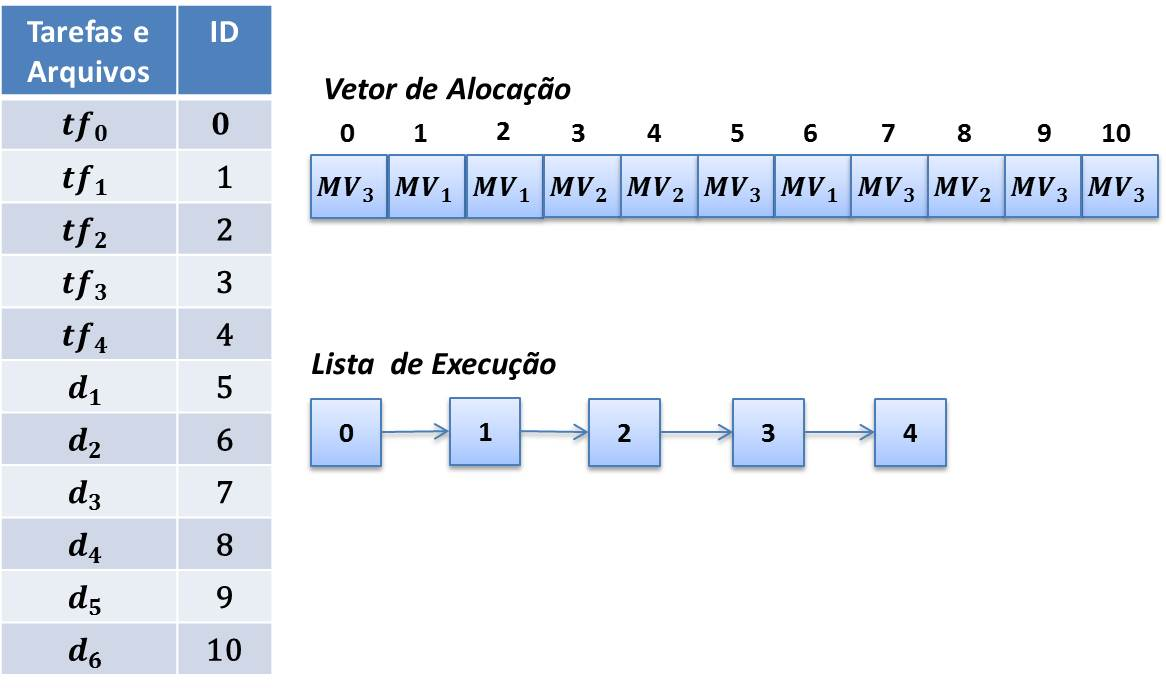
\includegraphics[width=1\linewidth]{figure/representacao.jpg}
        \caption{Estruturas de dados para representação do cromossomo.}
        \label{fig:encoding}
        \vspace{2\baselineskip}
    \end{subfigure}
    \begin{subfigure}{0.6\textwidth}
    \centering
        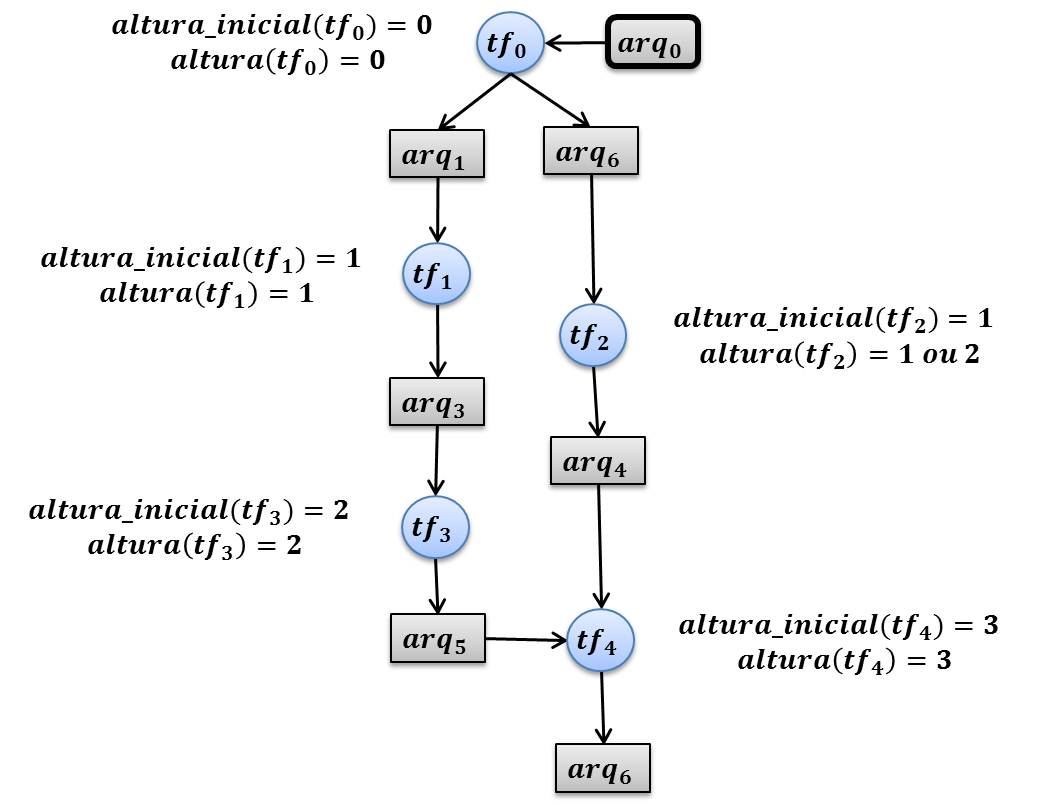
\includegraphics[width=0.9\linewidth]{figure/height.jpg}
        \caption{Cálculo da altura das tarefas.}
        \label{fig:height}
    \end{subfigure}
    \caption{Codificação do cromossomo.}
    \label{fig:representation}
    \end{figure}


A ordem de execução das tarefas é representada por uma lista encadeada chamada de \textit{lista de execução}, presente também  na Figura \ref{fig:encoding}. Para definir a ordem de execução das tarefas, um valor de altura é associado a cada uma delas. Uma tarefa só pode ser executada quando todas as tarefas de altura menores que a dela estiverem finalizadas. Já as tarefas com altura semelhante executam concorrentemente. O valor de altura é dado pelas equações \ref{eq:height}  e \ref{eq:heights}, propostas por Tsujimura e Gen \cite{Tsujimura1997}.

\begin{equation}
\label{eq:height}
\resizebox{0.8\textwidth}{!}
{
\text{$altura\_inicial(tf_i)$} = \begin{cases}
                            0, &\text{se } pred(tf_i) = \emptyset\\
                            1 + \max\limits_{tf_j \in pred(tf_i)}{altura\_inicial(tf_j)}, & \text{caso contrário}
                        \end{cases}
}
\end{equation}


\begin{equation}
\label{eq:heights}
\resizebox{0.8 \textwidth}{!} 
{
 
\text{$altura(tf_i)$}  = \begin{cases}
                altura\_inicial(tf_i),  &\text{se } suc(tf_i) = \emptyset\\
                    rand \in [altura\_inicial(tf_i), \min\limits_{\forall tf_k \in suc(tf_j)}{\{altura(tf_k)\}} - 1], &\text{caso contrário}
                  \end{cases}

}
\end{equation}


A equação \ref{eq:height} atribui para cada tarefa uma altura inicial correspondente ao nível no qual a tarefa aparece no grafo que representa o \textit{workflow}; a altura é zero quando não há predecessor, ou o máximo entre todas alturas iniciais de seus predecessores mais um. Essa equação permite que seja realizada uma ordenação topológica do grafo, já que basta definir grupos de tarefas de mesma altura (ou seja, que estão no mesmo nível) e, com base nos valores atribuídos, ordenar esses grupos de forma crescente. Porém, caso as tarefas sejam ordenadas apenas com base na altura inicial dada pela equação \ref{eq:height}, o paralelismo entre diferentes grupos de tarefas não seria explorado. Por exemplo, na Figura \ref{fig:height}, a tarefa $tf_2$ pode ser executada em paralelo tanto com $tf_1$ quanto com $tf_3$, pois não há relação de dependência entre essas tarefas. No entanto, a ordenação com base na altura inicial sempre atribuirá a altura de valor $1$ para $tf_2$, permitindo apenas o paralelismo entre $tf_2$ e $tf_1$. 

% At first, equation (\ref{eq:height}) assigns to a task an initial height corresponding to the order in which it can be executed; it can be zero when it has no predecessors, or the maximum of the initial heights among all predecessors plus one.

Para permitir que o paralelismo entre as tarefas seja totalmente explorado, um componente randômico é introduzido na equação \ref{eq:heights}. Esse componente permite que a tarefa possa ser executada em qualquer ordem entre a altura previamente calculada (altura inicial) e o valor mínimo da altura inicial de seus sucessores menos um. Seguindo o exemplo anterior, com o cálculo da Equação \ref{eq:heights} a tarefa $tf_2$  pode ser associada tanto ao valor $1$, sua altura inicial previamente calculada, quanto ao valor $2$, a altura de seu sucessor menos 1. Sendo assim, no caso em que o valor da altura de $tf_2$ for igual a $2$, a tarefa executaria em paralelo com $tf_3$. Dessa forma, diferentes sequencias de tarefas podem ser geradas para construir a \textit{lista de execução}. Essa característica é explorada pela função de \textit{crossover} e nos procedimentos de busca local, apresentados nas Subseções \ref{ssec:crossover} e \ref{ssec:localSearch}, respectivamente.


% After that, in equation (\ref{eq:heights}), a random component is introduced allowing that such task can execute in any order between the previous calculated height (initial height) and the minimum of heights among all its successors less one. For example, in Figure \ref{fig:height}, $task_2$ can be associated either to height equal $1$, its previous calculated height, or to height equal $2$, the height of its successor less one. Therefore, $task_2$ can run in parallel either with $task_1$ or $task_2$.

% Note that different sequences of tasks can be generated to encode the task execution order list. This feature is exploited in the search procedures as it will be seen in Subsections \ref{ssec:crossover} and \ref{ssec:localSearch}.

\subsection{População Inicial} \label{sssec:initialPopulation}

A população inicial é gerada por meio de duas abordagens distintas: (i) 80\% das soluções são geradas por heurísticas; e (ii) 20\% são geradas randomicamente.  As heurísticas MinMin \cite{minmin} e HEFT \cite{HEFT} foram utilizadas para gerar a primeira parte da população inicial. Como essas heurísticas são determinísticas, isto é, as mesmas soluções são produzidas para as mesmas entradas, cada solução gerada passa por um processo de mutação que seleciona aleatoriamente e altera uma porcentagem dos genes que compõe o cromossomo. Dessa forma, diferentes soluções são geradas a partir de uma única solução. 

Em primeiro lugar, 40\% das soluções são geradas a partir da solução produzida pelo MinMin, sendo que $\lambda\%$ dos genes no \textit{vector de alocação} são alterados randomicamente, onde $\lambda$ varia de 5\%  até 90\%. Em seguida, a mesma abordagem é utilizada para gerar os outros 40\% de cromossomos, porém, aplicada a solução produzida pelo HEFT. A ideia por trás dessa abordagem é garantir que a população inicial tenha uma diversidade satisfatória e represente um bom ponto de partida para a busca.


% To generate the initial population two approaches were applied. The first one uses both MinMin-TSH \cite{MINMIN} and HEFT \cite{HEFT} to generate 80\% of the initial population. Since these heuristics are deterministic and always produce the same solution to the same input, we applied a random component in each generated  solution to ensure that the population is diverse. Firstly, 40\% of solutions are generated from the solution produced by MinMin-TSH and we applied a random movement in $\lambda\%$ genes in the task and file assignment vector, where $\lambda$ ranges from 5\% to 100\% (increases in 5\% at each new solution). The same approach is used to generate the other 40\% of chromosomes, but at that point the chromosomes are derived from the solution produced by HEFT. The intuition behind this approach is that it ensures that initial population has a satisfactory diversified and presents a good start point to the search method.  

Para gerar os cromossomos restantes (20\% da população), cada tarefa e arquivo dinâmico é atribuído a uma MV randomicamente selecionada. A ordem de execução das tarefas é dada pela Equação \ref{eq:heights}, que é calculada para cada cromossomo gerado. Em ambas as abordagens, pode ocorrer de um arquivo dinâmico ser escalonado para uma MV que não tenha espaço de armazenamento suficiente. Quando isso ocorre, uma heurística proposta, chamada de \textit{move-arquivos}, é executada para realocar os arquivos dinâmicos de modo que a restrição de armazenamento não seja violada. A heurística \textit{move-arquivos} é apresentada na Subseção \ref{ssec:heuristic}.

% The second approach is used to generate the other 20\% of chromosomes. In that approach, each task and dynamic data file is assigned to a VM randomly chosen. The execution order of each task is given by (\ref{eq:heights}), that is calculated for each generated chromosome. 
% In both approaches, it may happen that a dynamic data file is assigned to a VM that does not have enough storage capacity to keep it. When it occurs, a proposed heuristic, named \textit{Move-file}, is executed to re-assign the dynamic files so that restriction is not violated. The heuristic \textit{Move-file} is presented in Subsection \ref{ssec:heuristic}.

\subsection{Operador de \textit{Crossover} e Fase de Seleção} \label{ssec:crossover}

A operação de \textit{crossover}, apresentada no Algoritmo \ref{algo:crossover}, combina dois indivíduos da população para formar um novo \textit{cromossomo}. No procedimento para gerar novas soluções (Algoritmo \ref{algo:doPop}), dois cromossomos da população atual \textit{P} são escolhidos utilizando o algoritmo de seleção por torneio \cite{Miller}. Em seguida, um operador de \textit{crossover} de recombinação em um ponto \cite{Holland1992} é aplicado em ambas as estruturas que compõem os cromossomos. Inicialmente, dois pontos de corte são definidos nas linhas \ref{l:corte1} e \ref{l:corte2} do Algoritmo \ref{algo:crossover}, um para o \textit{vetor de alocação} (\textit{corte1}) e outro para a \textit{lista de execução} (\textit{corte2}). Os genes à esquerda do \textit{corte1} são copiados do \textit{vetor de alocação} de $p1$ para as posições correspondentes da solução filho. Os genes restantes, posicionados à direita do corte, são copiados do \textit{vetor de alocação} de $p2$. Essa operação é também representada na Figura \ref{fig:crossover1}. Como pode ser visto, a solução resultante  contém uma parte das alocações originadas de $p1$ (representadas pela cor azul) e outra parte de $p2$ (cor verde). 

\begin{figure}[H]
\centering
\begin{subfigure}{.6\textwidth}
  \centering
  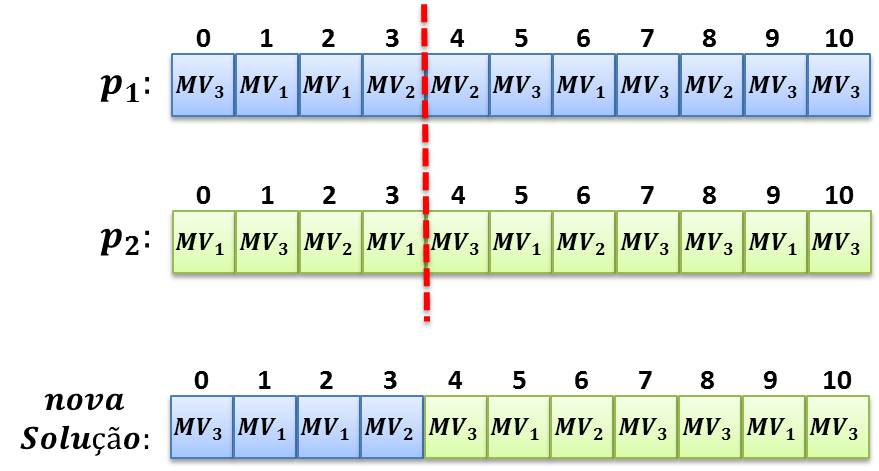
\includegraphics[width=1\linewidth]{figure/crossover1.jpg}
  \caption{\textit{Crossover} realizado no \textit{vetor de alocaçã}o.}
  \label{fig:crossover1}
  \vspace{2\baselineskip}
\end{subfigure}
\begin{subfigure}{.6\textwidth}
  \centering
  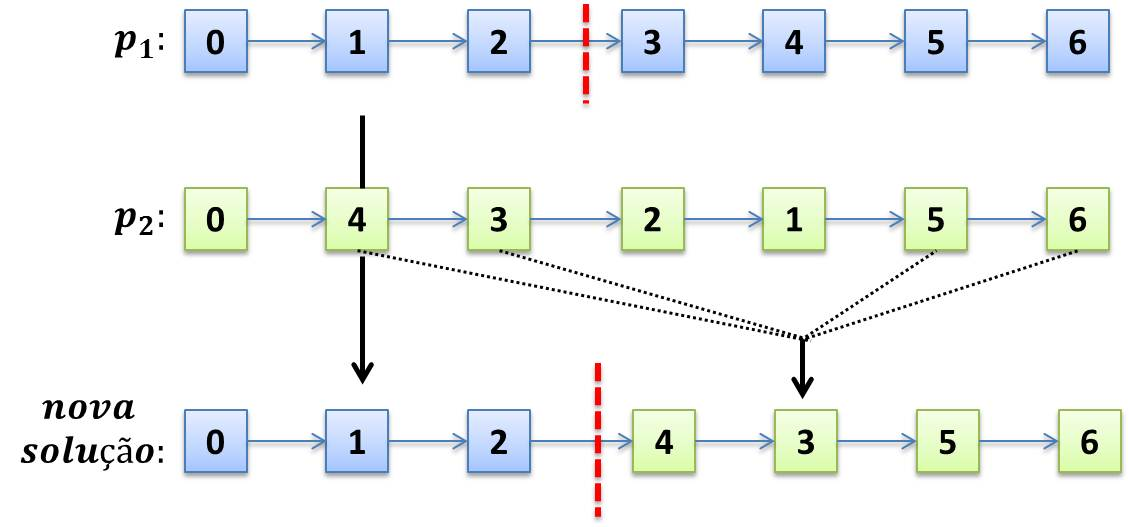
\includegraphics[width=1\linewidth]{figure/crossover2.jpg}
  \caption{\textit{Crossover} realizado na \textit{lista de execução}.}
  \label{fig:crossover2}
\end{subfigure}
\caption{Representação dos operadores de \textit{crossover} utilizados pelo AEH-ETAA.}
\label{fig:crossover}
\end{figure}


No caso do \textit{crossover} na \textit{lista de execução}, representado na Figura \ref{fig:crossover2} e presente nas linhas \ref{l:lista1} a \ref{l:lista2} do Algoritmo \ref{algo:crossover}, os genes do lado esquerdo do corte são copiados de $p_1$ para a solução filho (mantendo as mesmas posições). Já o restante dos genes da nova solução, são copiados da \textit{lista de execução} de $p_2$. Nesse último caso, as tarefas são verificadas uma a uma, e apenas as tarefas que ainda não estejam na solução filho são copiadas de $p_2$. Essa verificação é necessária para garantir que não haja repetição de tarefas, e assegurar que as ordens de precedência entre as tarefas sejam respeitadas.



\begin{algorithm}[H]
\caption{Procedimento \textit{Crossover}}\label{algo:crossover}

\begin{algorithmic}[1]
\Require Cromossomos $p1$ e $p2$.
\Ensure Novo Cromossomo (\textit{novo}).

    \State $corte1 \gets rand(1, |\textit{vetorAlocação}|)$\label{l:corte1}
    \State $corte2 \gets rand(1, |\textit{listaExecução}|)$\label{l:corte2}
    
    \For{$i \gets 1 \textbf{ a } |\textit{vetorAlocação}|$}
        \If{$i < corte1$}
            \State $novo.\textit{vetorAlocação}[i] \gets p1.\textit{vetorAlocação}[i]$
        \Else
            \State $novo.\textit{vetorAlocação}[i] \gets p2.\textit{vetorAlocação}[i]$        
        \EndIf
        
        \If{$i < corte2$} \label{l:lista1}
            \State $ novo.\textit{listaExecução} \gets novo.\textit{listaExecução} \cup p1.\textit{listaExecução}(i) $
        \EndIf
        
    \EndFor
    
    \For{$i \gets 1 \textbf{ a } |\textit{listaExecução}|$}
        \If{$p2.\textit{listaExecução}(i) \notin novo.\textit{listaExecução}$}            
            \State $ novo.\textit{listaExecução} \gets novo.\textit{listaExecução} \cup p2.\textit{listaExecução}(i) $
        \EndIf        
    \EndFor \label{l:lista2}

    
    \State \textbf{retorna} $novo$

\end{algorithmic}
\end{algorithm}

% Concerning the tasks execution order (Figure \ref{fig:crossover2}), genes from the left-hand side of the cut are copied from $parent_1$ to the genes of the same position of the offspring.
% The other genes of the offspring are obtained by checking each gene, in the same order they appear in $parent_2$, and copying it to the offspring whenever it has not been inserted in it yet. Thus, the precedence order of tasks is kept in the offspring.

Na fase de seleção (apresentada no Algoritmo \ref{algo:doPop}, linha \ref{l:selecaoInit} e \ref{l:selecaoFim}), os cromossomos da próxima população são selecionados a partir do conjunto chamado \textit{Soluções}, que é formado pelos novos cromossomos gerados e pela população anterior \textit{P}. Primeiro, para garantir que as melhores soluções sempre estarão incluídas na população, uma seleção elitista é aplicada na linha \ref{l:elitism}, na qual $5\%$ das melhores soluções são encontradas e adicionadas na próxima população \textit{P'}. Em seguida, as demais soluções são escolhidas utilizando o algoritmo de seleção por torneio e também são incluídas em \textit{P'}. Note que quando um cromossomo é selecionado ele é removido do conjunto \textit{Soluções} para prevenir que um mesmo cromossomo seja incluído mais de uma vez na população \textit{P'}.

\subsection{Operador de Mutação} \label{ssec:Mutation}

O operador de mutação é responsável pela diversificação da população, aumentando o espaço de busca e escapando dos chamados ótimos locais. Neste trabalho, o operador de mutação é executado apenas no \textit{vetor de alocação}. Os testes empíricos mostraram que a mutação aplicada à \textit{lista de execução} não apresenta melhorias significantivas em termos de qualidade da solução e, adicionalmente, aumenta o custo computacional do algoritmo.

 
A operação de mutação é chamada após o procedimento de \textit{crossover}, para cada nova solução gerada. Com base nas avaliações realizadas, fixou-se a probabilidade de mutação dos genes em $10\%$. Como pode ser visto na Figura \ref{fig:mutation}, o operador altera a identificação da MV aleatoriamente e, com isso, gera uma nova solução.
 
% The mutate operator is call for each new solution generated by the crossover procedure in the Algorithm \ref{algo:doPop}, on condition that each gene has a 10\% probability of being modified. As can be seen in Figure \ref{fig:mutation}, the VM identification \textit{Vm} is randomly changed. At the end, the fitness of the chromosome is recalculated and the new chromosome replaces the old one.


\begin{figure}[H]
	\center
  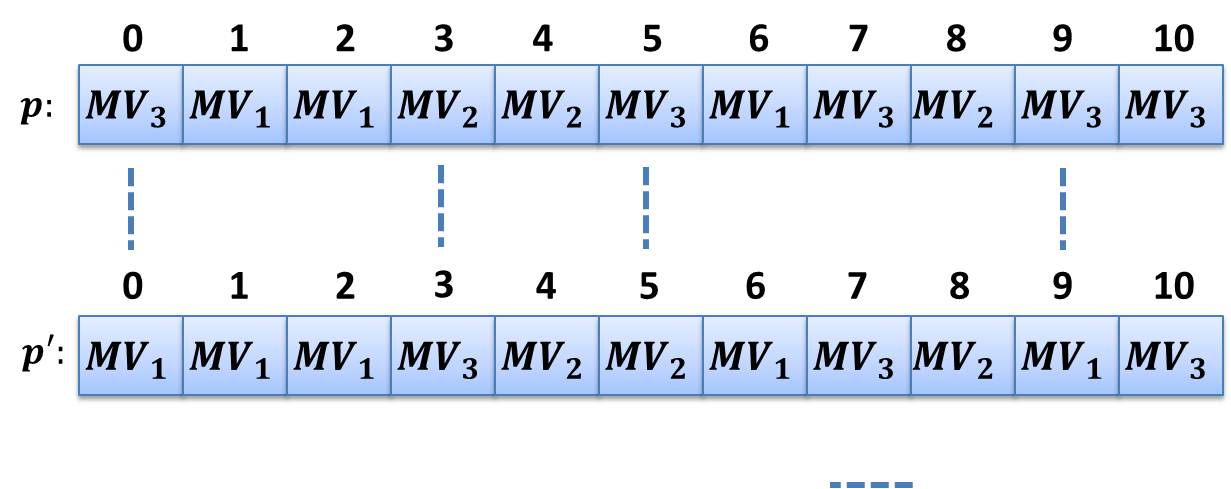
\includegraphics[width=0.6\linewidth]{figure/mutation.jpg}
  \caption{Operador de Mutação.}
  \label{fig:mutation}
\end{figure}

\subsection{Procedimentos de buscas locais} \label{ssec:localSearch}

Após a execução dos operadores de \textit{crossover} e mutação para construir a nova população, buscas locais são realizadas a $15\%$ das melhores soluções da população atual. As buscas locais ocorrem com uma probabilidade de $50\%.$ A porcentagem de soluções nas quais as buscas são realizadas e a probabilidade de ocorrência foram definidas através de testes empíricos feitos para ajustar os parâmetros do algoritmo. Como pode ser visto no Algoritmo \ref{algo:HEA} linha \ref{l:checkbl}, em cada iteração a probabilidade de busca local é verificada e, caso seja verdadeira, os procedimentos de buscas são executados.

Neste trabalho, três procedimentos de buscas locais foram definidos e são executados na seguinte ordem: (i) \textit{troca-mv} (Algoritmo \ref{algo:trocamv}), que executa a troca de dois elementos no \textit{vetor de alocação}; (ii) \textit{troca-posição} (Algoritmo \ref{algo:trocapos}), que troca a posição de dois elementos de mesma altura na \textit{lista de execução}; e (iii) \textit{move-elemento} (Algoritmo \ref{algo:moveelem}), que move uma tarefa ou um arquivo para uma MV diferente. Cada busca local é executada até que ocorra uma melhora na solução (primeira-melhora) ou até que todas as combinações sejam testadas.


\begin{algorithm}[H]
\caption{Procedimento \textit{troca-mv}}\label{algo:trocamv}

\begin{algorithmic}[1]
\Require Cromossomo $p$.
\Ensure Cromossomo $p$.
    
    \State $\textit{cópia} \gets p$
    
    \For{$i \gets 1 \textbf{ a } |\textit{vetorAlocação}|$}
        \For{$j \gets i + 1 \textbf{ a } |\textit{vetorAlocação}| $}
            \If{$p.\textit{vetorAlocação}[i] \neq p.\textit{vetorAlocação}[j]$}
                \State $troca(p.\textit{vetorAlocação}[i], p.\textit{vetorAlocação}[j])$
                \State $\textbf{calculaFitness}(p)$ \Comment{Algoritmo \ref{algo:fitness}.}
                \If{$ fitness(p) \textbf{ melhor que } fitness(\textit{cópia})$}
                    \State \textbf{retorna} $p$ 
                \Else
                    \State $troca(p.\textit{vetorAlocação}[i], p.\textit{vetorAlocação}[j])$ \Comment{Retorna ao estado anterior.}
                \EndIf                
            \EndIf
        \EndFor
    \EndFor    
    \State \textbf{retorna} \textit{cópia}
\end{algorithmic}
\end{algorithm}

\begin{algorithm}[H]
\caption{Procedimento \textit{troca-posição}}\label{algo:trocapos}

\begin{algorithmic}[1]
\Require Cromossomo $p$.
\Ensure Cromossomo $p$.
    
    \State $\textit{cópia} \gets p$
    
    \For{$i \gets 1 \textbf{ a } |\textit{listaExecução}|$}
        \State $tarefa_i \gets p.\textit{listaExecução}(i)$
        \For{$j \gets i + 1 \textbf{ a } |\textit{listaExecução}| $}
            \State $tarefa_j \gets p.\textit{listaExecução}(j)$
            \If{$altura(tarefa_i) = altura(tarefa_j)$}
                \State $troca(p.\textit{listaExecução}(i), p.\textit{listaExecução}(j))$
                \State $\textbf{calculaFitness}(p)$ \Comment{Algoritmo \ref{algo:fitness}.}
                \If{$ fitness(p) \textbf{ melhor que } fitness(\textit{cópia})$}
                    \State \textbf{retorna} $p$ 
                \Else
                    \State $troca(p.\textit{listaExecução}(i), p.\textit{listaExecução}(j))$ \Comment{Retorna ao estado anterior.}
                \EndIf                
            \Else
                \State \textbf{interrompe} \Comment{Interrompe laço e retorna ao laço externo.}
            \EndIf                
        \EndFor
    \EndFor    
    \State \textbf{retorna} \textit{cópia}
\end{algorithmic}
\end{algorithm}

\begin{algorithm}[H]
\caption{Procedimento \textit{move-elemento}}\label{algo:moveelem}

\begin{algorithmic}[1]
\Require Cromossomo $p$.
\Ensure Cromossomo $p$.
    
    \State $\textit{cópia} \gets p$
    
    \For{$i \gets 1 \textbf{ a } |\textit{vetorAlocação}|$}
        \State $\textit{MV\_atual} \gets p.\textit{vetorAlocação}[i]$
        \For{$\textit{MV\_prox} \gets  1 \textbf{ a } \textit{NÚMERO\_MVs} $}
            \If{$\textit{MV\_atual} \neq \textit{MV\_prox}$}
                \State $p.\textit{vetorAlocação}[i] = \textit{MV\_prox}$
                \State $\textbf{calculaFitness}(p)$ \Comment{Algoritmo \ref{algo:fitness}.}
                \If{$ fitness(p) \textbf{ melhor que } fitness(\textit{cópia})$}
                    \State \textbf{retorna} $p$ 
                \Else
                    \State $p.\textit{vetorAlocação}[i] = \textit{MV\_atual}$ \Comment{Retorna ao estado anterior.}
                \EndIf                
            \EndIf
        \EndFor
    \EndFor    
    \State \textbf{retorna} \textit{cópia}
\end{algorithmic}
\end{algorithm}


\begin{figure}[H]
\centering
\begin{subfigure}[t]{.5\textwidth}
  \centering
  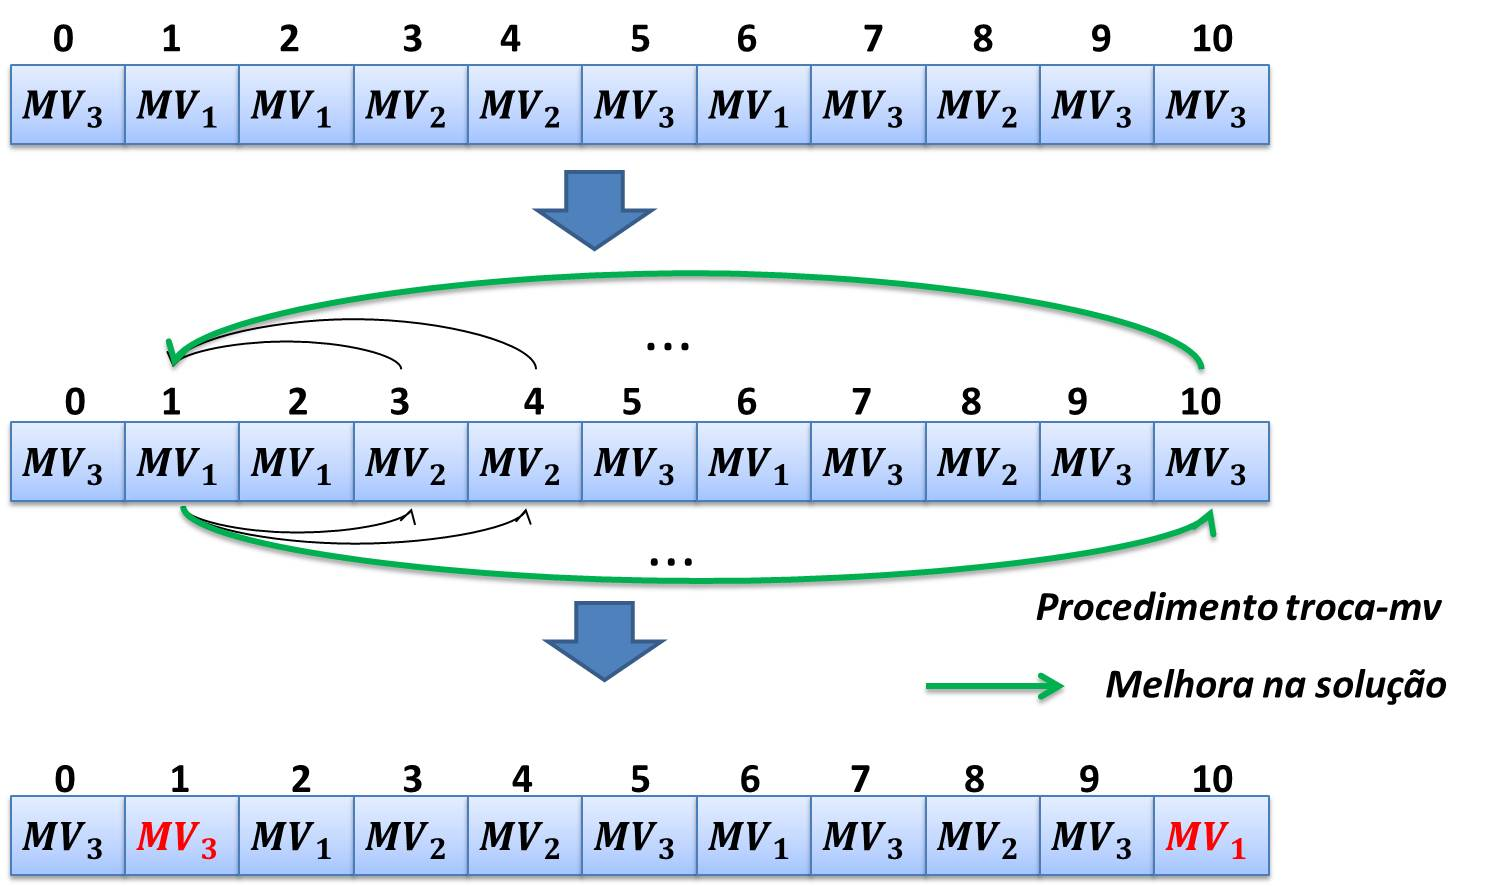
\includegraphics[width=1\linewidth]{figure/swap_vm.jpg}
  \caption{Troca de máquinas no \textit{vetor de alocação}.}
  \label{fig:swapvm}
\end{subfigure}%
\begin{subfigure}[t]{.5\textwidth}
  \centering
  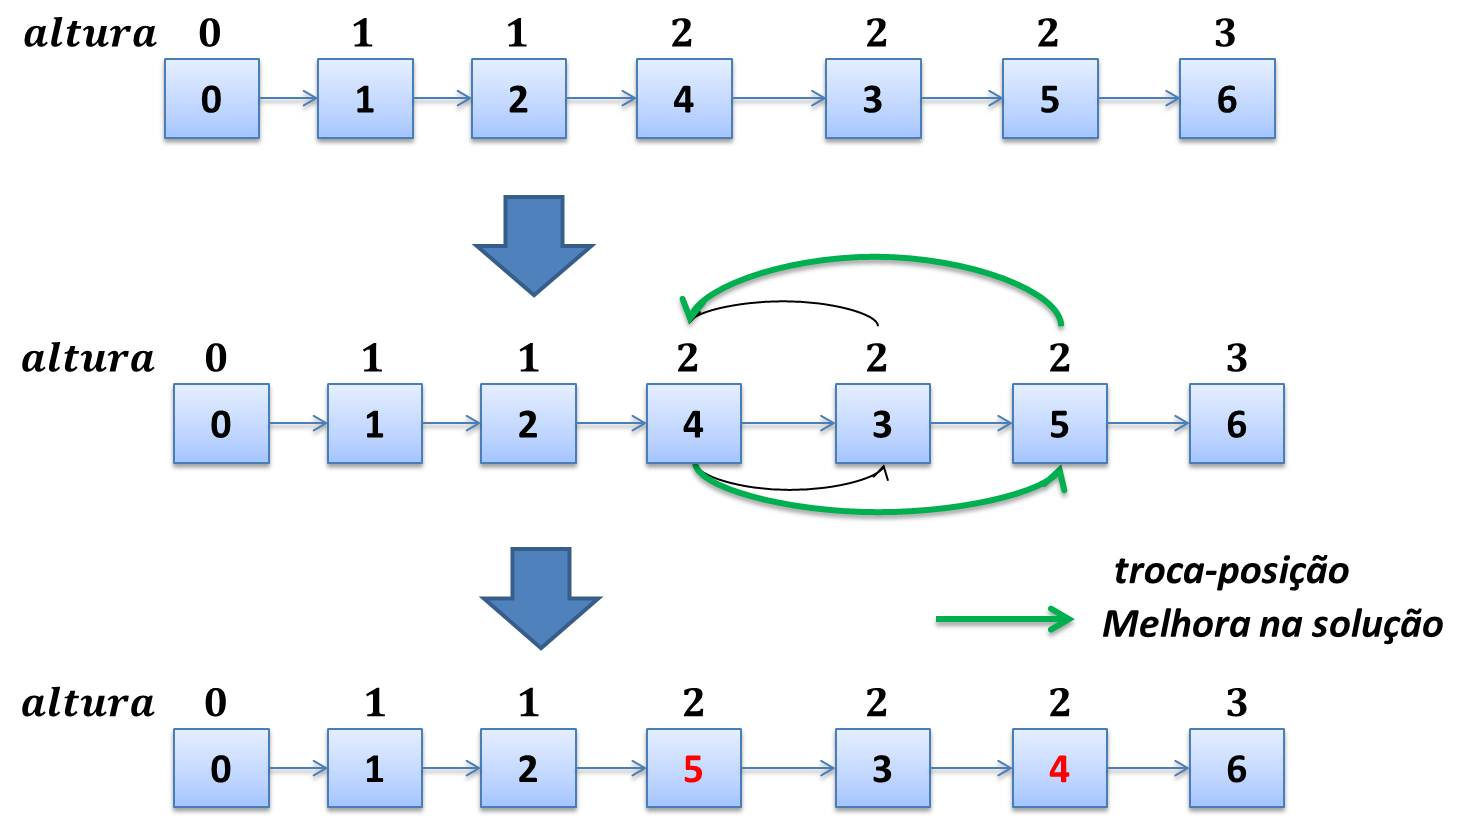
\includegraphics[width=1\linewidth]{figure/swap_sequence.jpg}
  \caption{Troca de tarefas na \textit{lista de execução}.}
  \label{fig:swapsequence}
\vspace{1\baselineskip}
\end{subfigure}
\begin{subfigure}{.5\textwidth}
  \centering
  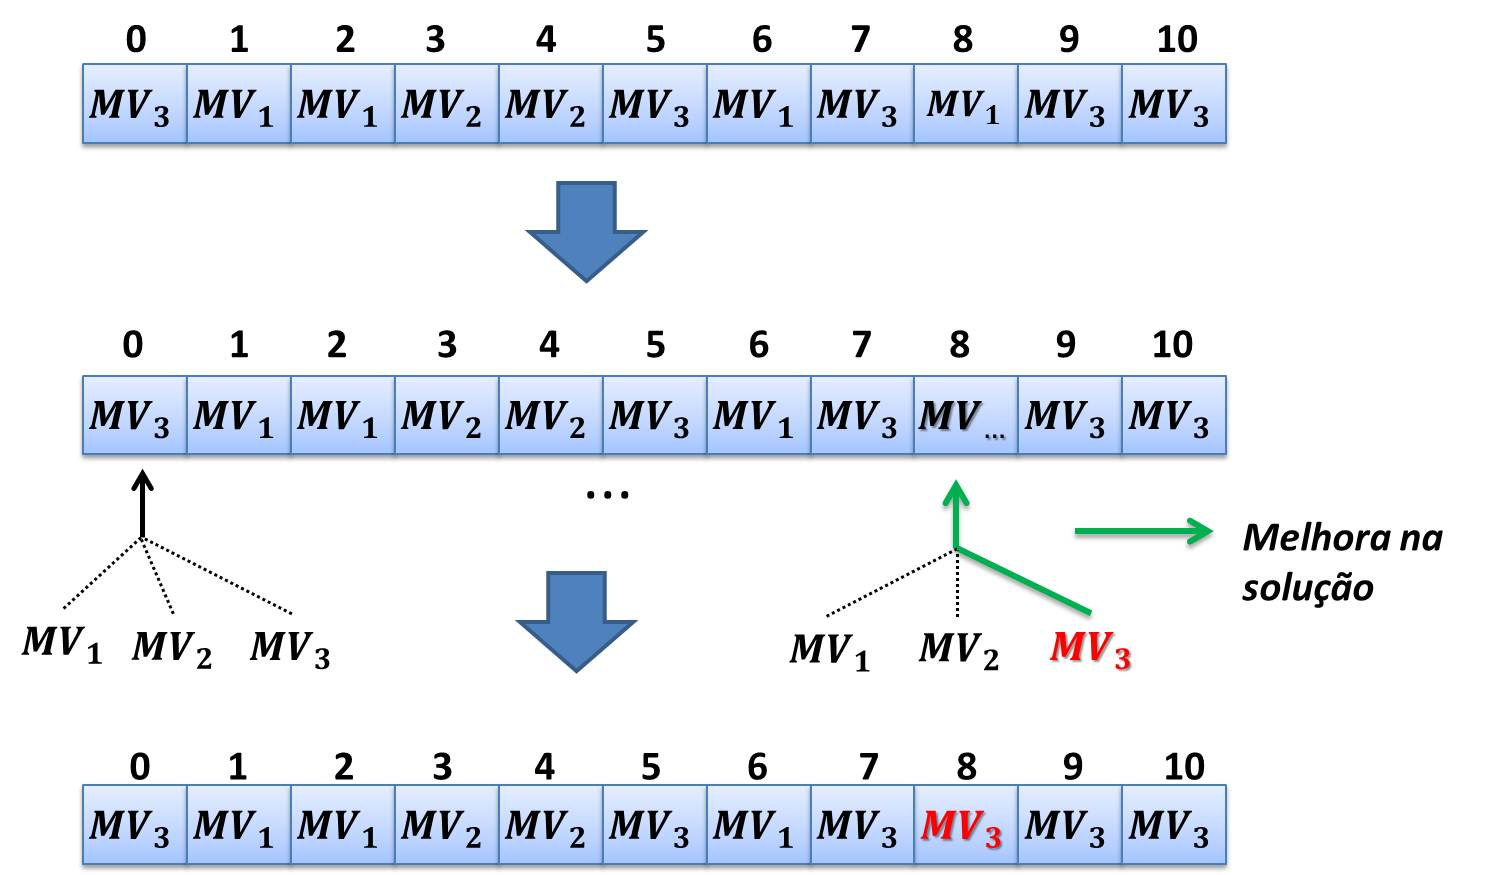
\includegraphics[width=1\linewidth]{figure/move_element.jpg}
  \caption{Move uma tarefa ou um arquivo de uma máquina para outra.}
  \label{fig:move}
\end{subfigure}
\caption{Procedimentos de Buscas Locais Implementados.}
\label{fig:localSearch}
\end{figure}



A Figura \ref{fig:localSearch} apresenta os três tipos de buscas locais utilizadas no AEH-ETAA. A Figura \ref{fig:swapvm} mostra a execução do procedimento \textit{troca-mv} que, após testar vários movimentos, troca os elementos da posição 1 e 10 do \textit{vetor de alocação}. A Figura \ref{fig:swapsequence} também executa várias trocas, até mover a ordem de execução da tarefa 4 e 5, que apresentam a mesma altura na \textit{lista de execução}. Por fim, na Figura \ref{fig:move}, a tarefa ou o arquivo é movido da $MV_2$ para $MV_3$.

\subsection{\textit{Path Relinking}}\label{ssec:pr}

\textit{Path relinking} é uma heurística capaz de gerar soluções intermediárias entre duas outras soluções. O operador começa com uma solução inicial e, passo a passo, insere elementos de uma solução guia. O objetivo é visitar novas soluções no caminho traçado entre uma solução e outra \cite{Glover2000}. Portanto, durante a execução do \textit{path relinking}, a distância entre as soluções diminui gradualmente.

% Path relinking is a heuristic capable of generating intermediate solutions between two other ones.
% It starts with an initial solution and, step by step, inserts elements of a target solution. Its goal is to visit new solutions in the path from one solution to another one \cite{Glover2000}.
% So, during the path relinking execution, the distance between the solutions diminishes gradually.

Neste trabalho, a distância de um cromossomo $p_i$ em relação a um cromossomo $p_j$ é dada pela soma do número de elementos (tarefas ou arquivos) alocados a diferentes MVs, com o número de movimentos necessários para que a \textit{lista de execução} de $p_i$ seja semelhante a de $p_j$. A Figura \ref{fig:distance} mostra a distância entre os cromossomos $p_1$ e $p_2$. Como pode ser visto, o número de tarefas e arquivos alocados em diferentes MVs é $5$ e apenas um movimento é necessário na \textit{lista de execução}, portanto $dist(p_1, p_2) = 6$.

% In the context of TaSDAP, the distance between a chromosome $chr_1$ and another $chr_2$ is the number of tasks and data files assigned to different VMs plus the number of swaps necessary to turn their task order lists exactly the same. Figure \ref{fig:distance} shows the distance of  chromosomes  $chr_1$ and $chr_2$.  The  number of tasks or data files placed in different VMs is five and the number of necessary swaps is one, so $dist(chr_1, chr_2) = 6$.

%\begin{figure}[H]
%	\center
%  \includegraphics[width=70mm,scale=0.9]{figure/distance.jpg}
%  \caption{Distance $dist(chr_1, chr_2) = 6$}
%  \label{fig:distance}
%\end{figure}

\begin{figure}[H]
\centering
\begin{subfigure}{.5\textwidth}
  \centering
  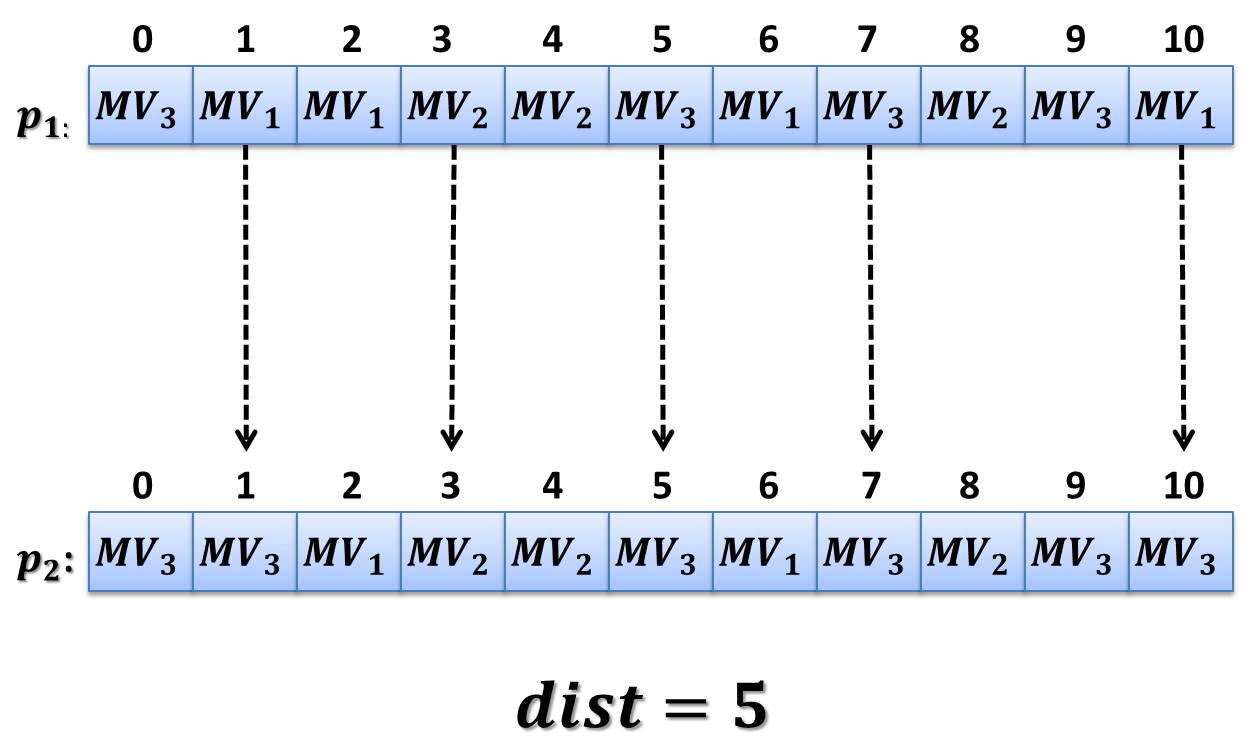
\includegraphics[width=.9\linewidth]{figure/distance1.jpg}
 \end{subfigure}%
\begin{subfigure}{.4\textwidth}
  \centering
  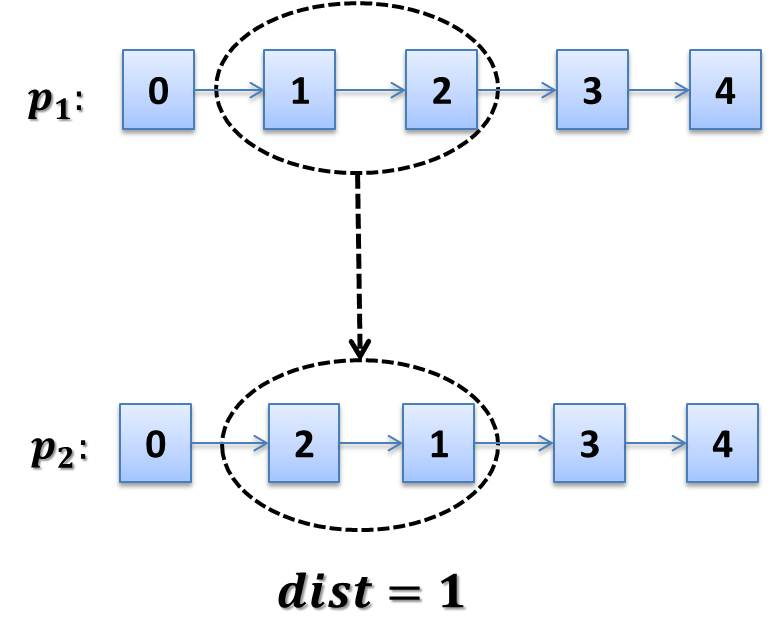
\includegraphics[width=.9\linewidth]{figure/distance2.jpg}
\end{subfigure}
\caption{Cálculo da distância entre os cromossomos $p_1$ e $p_2$, $dist(p_1, p_2) = 6$}
\label{fig:distance}
\end{figure}

O \textit{path relinking} é aplicado quando uma melhor solução (\textit{best}) é encontrada no procedimento principal (Algoritmo \ref{algo:HEA}, linha \ref{l:path1}). Como pode ser visto no Algoritmo \ref{algo:pr}, as soluções presentes no conjunto elite atuam como pontos iniciais da busca (chamados de \textit{origem}). O conjunto elite é composto pelas melhores soluções cuja distância entre cada uma delas é maior que $\alpha$, onde $\alpha$ é calculado como $25\%$ do número de tarefas e arquivos do \textit{workflow}. Esse parâmetro controla a diversidade do conjunto e, consequentemente, a eficiência da busca. Além disso, para controlar o número de buscas efetuadas, um limite máximo de $\beta$ cromossomos é definido para o conjunto elite, sendo que o valor de  $\beta$ é igual a metade do tamanho da população. Quando esse limite é alcançado, uma política de substituição \textit{First-in First-out} (FIFO) é aplicada para substituir a solução mais antiga pela mais nova. 
 
 \begin{algorithm}
 \caption{Procedimento \textit{PathRelinking}}\label{algo:pr}
 
 \begin{algorithmic}[1]
\Require Cromossomo $destino$ e Conjunto Elite $ConjElite$.
\Ensure Melhor cromossomo encontrado ($best$).
    
    \State $best \gets destino$
    
    \For{$cont \gets 1 \textbf{ a } |\textit{ConjElite}|$}
    
        \State $\textit{origem} \gets ConjElite(cont)$
                
        \For{$i \gets 1 \textbf{ a } |origem.\textit{vetorAlocação}|$} \label{l:prlaco}
            \If{$origem.\textit{vetorAlocação}[i] \neq destino.\textit{vetorAlocação}[i]$}
                \State $origem.\textit{vetorAlocação}[i] \gets destino.\textit{vetorAlocação}[i]$
                \State $\textbf{calculaFitness}(origem)$ \Comment{Algoritmo \ref{algo:fitness}.}
                \If{$fitness(origem) \textbf{ melhor que } fitness(best)$}
                    \State $best \gets origem$ \label{l:updatebest}
                \EndIf  
            \EndIf
        
        \EndFor
        
    \EndFor    
    \State \textbf{ retorna } $best$
\end{algorithmic}
\end{algorithm}


Como visto no Algoritmo \ref{algo:pr}, a busca se concentra no \textit{vetor de alocação} das soluções. A cada iteração do algoritmo (linha \ref{l:prlaco}), um elemento do \textit{vetor de alocação} da solução \textit{destino} é copiado para o vetor da solução origem. Na sequencia, o valor de \textit{fitness} da solução resultante é comparado com o melhor resultado obtido (armazenado em \textit{best}) e, caso o valor seja melhor, o \textit{best} é atualizado (linha \ref{l:updatebest}). Essas etapas são repetidas para cada um dos cromossomos do conjunto elite e, por fim, a melhor solução encontrada é retornada para o procedimento principal.
 
\subsection{Heurística \textit{move-arquivos}} \label{ssec:heuristic}

Quando um novo cromossomo é gerado sua viabilidade é avaliada. Se os arquivos alocados a uma MV excedem sua capacidade de armazenamento, a MV é considerada sobrecarregada e a heurística \textit{move-arquivos} é executada.

% When a new chromosome is generated, its feasibility is evaluated. If the data files assigned to a VM exceed its storage capacity, the VM is considered overloaded and the heuristic \textit{Move-file} is executed.

A heurística contém as seguintes etapas:
\begin{enumerate}
\item Seleciona a MV mais sobrecarregada, $MV_s$.
\item Selecione a MV com maior quantidade de espaço livre, $MV_d$.
\item Move o arquivo de menor tamanho alocado em $MV_s$ para $MV_d$.
\end{enumerate}

% The heuristic \textit{Move-file} contains the following steps: 
% \begin{enumerate}
% \item  Select the most overloaded VM, $m_s$.
% \item  Select the most underloaded VM, $m_d$.
% \item  Move the smallest size data file from VM $m_s$ to $m_d$.
% \end{enumerate}

Os passos acima são repetidos até que não haja MVs sobrecarregadas.

% The above  steps are repeated until there is no overloaded VM.

Baseado na hipótese de que as alocações definidas pela metaheurística correspondem as melhores alocações possíveis, parece razoável não modificar muito o cromossomo original, já que isso pode impactar o \textit{makespan} resultante. Para minimizar esse provável impacto, os arquivos de menor tamanho são selecionados para serem movidos.

% Based on the hypothesis that the assignments defined by the metaheuristic correspond to the best ones, it seems interesting not changing the original chromosome very much, since it could impact negatively on the makespan. In order to soften this probable impact, the smallest data files are selected to be moved.

\subsection{Função de \textit{fitness}} \label{ssec:fitness}

A função de \textit{fitness} pode ser definida como $f: s \rightarrow Z$, onde $s$ é uma solução viável do espaço de busca e $Z$ é um número inteiro que quantifica a qualidade da solução representada pelo cromossomo. Portanto, a função de \textit{fitness} permite ordenar as soluções em termos de qualidade e direcionar a busca para as melhores soluções \cite{Talbi2009}.

% Let $f: s \rightarrow Z$ be a fitness function, where $s$ is a feasible solution in the search space and $Z$ is an integer number that quantifies the quality of a solution represented by a chromosome. So, the fitness function allows for ordering the solutions in terms of quality and to direct the search towards the best solutions \cite{Talbi2009}.

Neste trabalho, a qualidade de um indivíduo é dada pelo \textit{makespan}, \textit{i.e.}, seja $p_i$ e $p_j$ dois cromossomos, se $makespan(p_i) < makespan(p_j)$, então a solução dado por $p_i$ é melhor que a dada por $p_j$. Ou seja, a função de \textit{fitness} se resume ao cálculo do \textit{makespan} associado a cada solução. O Algoritmo \ref{algo:fitness} efetua esse cálculo. Como pode ser visto, as informações da \textit{lista de execução} e do \textit{vetor de alocação} são utilizadas para estimar o tempo final de cada tarefa.

% In TaSDAP, the quality of an individual is given by the makespan, \textit{i.e.}, let $chr_i$ and $chr_j$ be two chromosomes, if $makespan(chr_i) < makespan(chr_j)$, then the solution given by $chr_i$ is better than the one given by $chr_j$. To calculate the makespan, we define the Algorithm \ref{algo:fitness}. As can be seen, the information in the structures \textit{order list} (sorting by the tasks height values) and \textit{assignment vector} are retrieved to compute the finish time of each task.  

\begin{algorithm}[H]
\caption{Procedimento \textit{CalculaFitness}}\label{algo:fitness}

\begin{algorithmic}[1]
\Require \textit{Vetor de Alocação} e \textit{Lista de Execução}.
\Ensure Valor do \textit{Makespan}.

    \State $Q \gets 0$ 
    \State $FT \gets 0$
    \For{$tf_i$ \textbf{em } $\textit{listaExecução} $}
        \State $MV_j \gets \textit{vetorAlocação}[tf_i]$
        \State $t\_max\_pred \gets maxTempoFinalPred(FT, tf_i)$
        \State $t\_inicial_i \gets \max{(t\_max\_pred, Q[MV_j])} $ \label{l:inicial}
        \State $t\_final_i \gets t\_inicial_i + \text{execução}(tf_i, MV_j) + leitura(tf_i) + escrita(tf_i)$ \label{l:final}
        \State $Q[vm_j] \gets t\_final_i$
        \State $FT[tf_i] \gets t\_final_i$
    \EndFor

    \State \textbf{retorna} $\max(FT)$ \label{l:fitretorno}


\end{algorithmic}
\end{algorithm}

No Algoritmo \ref{algo:fitness}, os vetores \textit{Q} e \textit{FT} são estruturas auxiliares usadas para manter o tempo calculado em cada etapa do algoritmo. O vetor \textit{Q} é indexado pelo identificador da máquina  e contém o tempo final da última tarefa executada na MV correspondente. Já o vetor \textit{FT} armazena o tempo final de cada tarefa $tf_i$, utilizada como índice do vetor.

% In Algorithm \ref{algo:fitness}, vectors \textit{Q} and \textit{FT} are auxiliary structures used to keep the times computed in every step of the algorithm.  Vector  \textit{Q}  is indexed by the VM identification ($m_j$) and  contains the finishing time of the last task executed in the corresponding VM. Each element of   vector \textit{FT}  corresponds to a $task_i$ and  contains the finishing time of  the associated task.

Os cálculos de tempo inicial e final de cada tarefa seguem o modelo apresentado na Subseção \ref{sec:problemDef}. Primeiramente, o tempo inicial da tarefa $tf_i$ é computado como o máximo entre os tempos finais de seus predecessores imediatos (representado por \textit{t\_max\_pred}) e o tempo final da ultima tarefa executada na $MV_j$ (armazenado em $Q[MV_j]$), como apresentado na linha \ref{l:inicial}.

% The calculations of the start and  finishing times  of each task follows the model presented in Subsection \ref{sec:problemDef}. Firstly, the start time of $task_i$  is  computed as the the maximum finishing time among all its  immediate predecessors (represented by  \textit{max\_pred\_time}) and the finishing time of the last task executed in VM $m_j$ (stored in $Q[m_j]$), as presented in line 6. 

Em seguida, na linha \ref{l:final}, o tempo final da tarefa $tf_i$ é calculado como a soma dos seguintes valores: (i) o tempo inicial de $tf_i$ ($t\_inicial_i$); (ii) o tempo de execução de $tf_i$ quando executada na $MV_j$; (iii) o tempo necessário para ler todos os dados de entrada de $tf_i$; e (iv) o tempo necessário para escrever todos os arquivos gerados por $tf_i$. Finalmente, na linha \ref{l:fitretorno}, o algoritmo retorna o valor de \textit{makespan}.

% Then, in  line 7, the finishing time of $task_i$ is computed by summing the following values: (i) the start time of $task_i$ ($start\_time_i$); (ii) the execution time of $task_i$ when executed in VM $m_j$; (iii) the  necessary time for reading all required data files by  $task_i$; and (iv) the  necessary time  for writing all data files generated by $task_i$. Finally, in line 10, the algorithm returns the makespan that  is  the maximum finishing time among all tasks of the workflow.


